\documentclass[tikz,border=4pt]{standalone}
\usetikzlibrary{positioning, arrows.meta}

\tikzset{
  neuron/.style      = {draw, thick, circle, minimum size=8mm, inner sep=0pt},
  input/.style       = {neuron, fill=gray!12},
  hidden/.style      = {neuron, fill=blue!10},
  output/.style      = {neuron, fill=orange!20},
  layer title/.style = {font=\small\bfseries, align=center},
  weight/.style      = {->, draw=black!45},
  >={Stealth[length=2mm]},
}

\begin{document}
% A small fully connected network: 3 inputs, 4 hidden units, 2 outputs.
% "on grid" measures node distances between centers, so the layers line up.
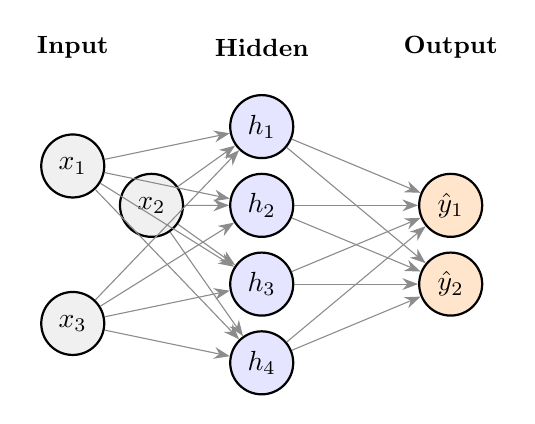
\begin{tikzpicture}[node distance=10mm and 24mm, on grid]
  \node[input]                             (x1) {$x_1$};
  \node[input, below right=5mm and 1cm of x1]                (x2) {$x_2$};
  \node[input, below=2cm of x1]                (x3) {$x_3$};

  \node[hidden, above right=5mm and 24mm of x1] (h1) {$h_1$};
  \node[hidden, below=of h1]               (h2) {$h_2$};
  \node[hidden, below=of h2]               (h3) {$h_3$};
  \node[hidden, below=of h3]               (h4) {$h_4$};

  \node[output, right=of h2]               (y1) {$\hat y_1$};
  \node[output, right=of h3]               (y2) {$\hat y_2$};

  \node[layer title, above=15mm of x1]     (input)  {Input};
  \node[layer title, above=10mm of h1]     (hidden) {Hidden};
  \node[layer title, above=20mm of y1]     (output) {Output};

  % Every input to every hidden unit, then every hidden unit to every output.
  \draw[weight] (x1) -- (h1);
  \draw[weight] (x1) -- (h2);
  \draw[weight] (x1) -- (h3);
  \draw[weight] (x1) -- (h4);
  \draw[weight] (x2) -- (h1);
  \draw[weight] (x2) -- (h2);
  \draw[weight] (x2) -- (h3);
  \draw[weight] (x2) -- (h4);
  \draw[weight] (x3) -- (h1);
  \draw[weight] (x3) -- (h2);
  \draw[weight] (x3) -- (h3);
  \draw[weight] (x3) -- (h4);
  \draw[weight] (h1) -- (y1);
  \draw[weight] (h1) -- (y2);
  \draw[weight] (h2) -- (y1);
  \draw[weight] (h2) -- (y2);
  \draw[weight] (h3) -- (y1);
  \draw[weight] (h3) -- (y2);
  \draw[weight] (h4) -- (y1);
  \draw[weight] (h4) -- (y2);
\end{tikzpicture}
\end{document}
